\documentclass{article}

\usepackage{amsmath}
\usepackage{graphicx}
\usepackage[colorlinks=true]{hyperref}

\title{MP1 \\ CS 598: Parallel Migratable Objects}
\author{Fall 2014}
\date{Due date: Tuesday, September 23, 10 PM}

\begin{document}
\maketitle

\textbf{Description:} 
Parallel prefix can be used to implement a load balancing strategy. In this
assignment, you will implement a load balancer using parallel prefix. You
can implement the parallel prefix Charm++ program given in the class slides or
can implement your own version. 

%For this assignment you need to write a Charm++ program which does manual load
%balancing of integer numbers among elements of a 1D chare array using the 
%given parallel prefix code in the class slides or with your own parallel 
%prefix code. 

To implement the parallel prefix program, create a chare array of size $s$. Each
chare array element, $i$, generates $n_i$ random integers where the value of
$n_i$ is randomly generated between $min$ and $max$. The set of numbers generated
can be stored in an array or stl vector. Your program takes $min$,
$max$ and $s$ as the command line arguments. Use $rand()$ to generate random
numbers. This can create load imbalance depending on the value of $n_i$, which is
the number of integers $i^{th}$ chare array element owns. Perform manual load
balancing using parallel prefix so as to distribute the numbers such that each
chare array element owns approximately  $\frac{n}{s}$ integers where  $n = n_1 +
n_2 \cdots n_s$.\\


%First, you create a chare array of size $s$, where each chare $i$ in the chare array generates 
%(and hence owns) $n_i$ integer numbers. For every chare $i$, $n_i$ is a 
%randomly generated number between $min$ and $max$. 
%$min$, $max$ and $s$ are command line parameters. 
%Once $n_i$ is generated, chare $i$ generates $n_i$ random 
%integers (using rand()). In other words, each chare is creating a random number(between $min$ and $max$), and then creating that many more random numbers(not bounded). You can store the integers in a simple array or a stl vector. The task is to load balance the count
%of integer number among chares, i.e. if $n = n_1 + n_2 \cdots n_s$,
%each chare should get approximately $\frac{n}{s}$ integers. \\

The prefix sum and the average elements per chare array element is used to
determine which chare array elements need to send which integer elements.  To
obtain the average number of integers per chare array element, use reductions.
See
\href{http://charm.cs.uiuc.edu/manuals/html/charm++/4.html#SECTION01361000000000000000}{Charm++
reductions manual section} for details on reductions. Figure~\ref{prefix} gives
an example of how load balance can be achieved. 

%Use reduction to get the average number of integers per chare. (See \href{http://charm.cs.uiuc.edu/manuals/html/charm++/4.html#SECTION01361000000000000000}{ Charm++ reductions manual section}.) The average should be useful in deciding which integers should be at which chares
%after load balancing. Use exclusive parallel prefix (count of integers in chare $i$
%is not counted in $prefix_i $) to decide which chare array element 
%should send which integers to which chare array element. Figure~\ref{prefix}
%may provide hints. \\


\begin{figure}[h]
\centering
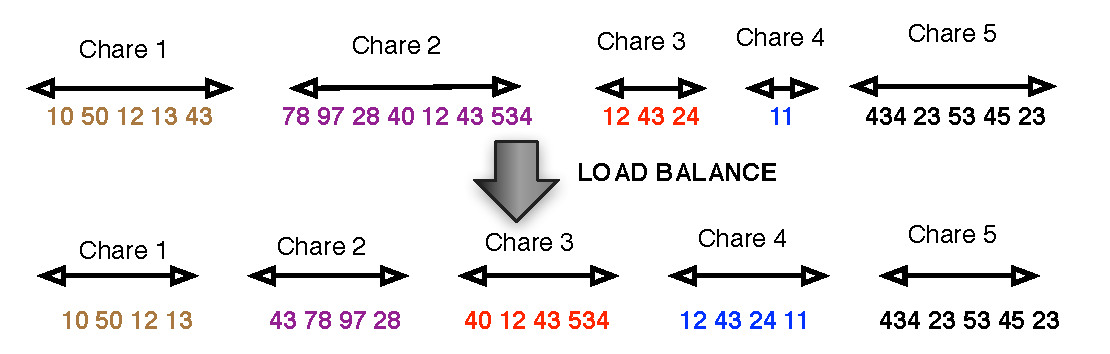
\includegraphics[width=\textwidth]{prob1.pdf}
\caption{Load balancing integers among chares.}
\label{prefix}
\end{figure}


\textbf{Detailed Algorithm:} 

\begin{enumerate}

\item Create a chare array of size $s$ and initialize the integer elements on
each chare array element. Chare array element $i$ contains $n_i$ random integers
where $n_i$ is a random number between $min$ and $max$. $min$,
$max$ and $s$ are input arguments to your program.
%\item  Create the initial integer elements on all chares

\item Execute the parallel prefix code on number of elements in a chare array
element, $n_i$, to obtain the prefix sum. Let $p_i$ contain the prefix sum on
chare array element at index $i$ where $p_i = \sum\limits_{k=0}^{i-2} n_k$.
%\item On every chare, execute code to find prefix sum of number of elements ($p_i$ on chare $i$)

\item Find average number of elements, $avg$, either using reduction or using prefix sum.

\item Once you have the prefix sum, $p_i$, and $avg$, data exchange to load
balance can be done as follows
\begin{itemize}
\item consider a logical ranking of the elements $0$ to $(n-1)$.
\item in a balanced distribution, elements with ranks $avg*i$ to $avg*(i +1)-1$ will reside on chare $i$
\end{itemize}

%\item Find average number of elements either using reduction or information from prefix sum (say avg).
%Data exchange to load balance can be done as follows:
%\begin{itemize}
%\item consider a logical ranking of the elements 1 to n where ranks 0 to $N_1$ - 1 are on chare 1, $N_1$ to $N_2-1$ are on chare 2, and so on..
%\item in the load balanced distribution, elements with ranks $avg*i$ to $avg*(i +1)-1$ will reside on chare $i$
%\end{itemize}

\item Every chare array element identifies the rank for the integer elements it
owns. For chare array element $i$, the ranks of the elements it contains would
range from $p_i$ to $p_i + (n_i - 1)$. Integer element with $rank_j$ should be
sent to chare array element with index $floor(j/avg)$. Send these elements to
the correct destination using messages. Also send the starting rank so that the
destination can place these elements in the right location in the array. Do not
send the elements in separate messages instead bunch them up together so that
all the elements from a chare array element that needs to be sent to a
destination is sent in one single message.

%\item On every chare which initially contains elements with ranks $p_i$ to $p_(i+1) - 1$, find the final destination of the elements (element with rankj should go to chare $floor(j/avg)$ ) and send them to the destination chares (also send their starting rank, so the detination can store it in the right place). Do not send individual values in separate messages.. bunch together all the data chare $x$ sends to chare y in a single method invocation.

\item On receiving a message, every chare array element copies these new
elements in a new list in their correct position (using the ranks)
%\item On every chare, receive the incoming messages and copy them to a new element list in their correct position (using the ranks)
 
\end{enumerate}

\emph{Correctness Test}: The checksum of the integers in the beginning
should be same as checksum of the integers after the load balancing
Use \emph{bitvec\_xor} operation of the integers to compute checksum in  \href{http://charm.cs.uiuc.edu/manuals/html/charm++/4.html#SECTION01361000000000000000}{ Charm++
reductions}. \\

\emph{Exit condition}: You can either use Quiescence Detection (with CkStartQD(..) function, for more
information about QD go to related
\href{http://charm.cs.illinois.edu/manuals/html/charm++/12.html#SECTION02350000000000000000}{manual
section}) to terminate or your own method to detect when
the load balancing is complete. \\


\textbf{Running your code:}
The program should have the following signature: \\
\textit{./charmrun ./mp1 +p4 chare-array-size min max} \\

You should test your code on Taub cluster up to 64 nodes. You can start with a small
number of processors and once you make sure your algorithm works, you can test
with more number of processors. You can use 1024 as
\textit{chare-array-size} and \textit{min/max} could be in the range of [5,000 - 30,000].
\\ \\ \\

%\pagebreak

\textbf{A Case Study:} 

\begin{figure}[h]
\centering
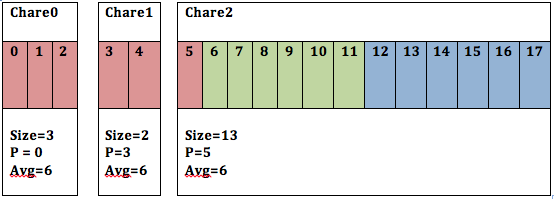
\includegraphics[width=\textwidth]{before_balance.png}
\caption{Before load balancing.}
\label{prefix}
\end{figure}

After load balancing, all the reds will be in Chare 0, all greens in Chare 1, all blues in Chare2. \\
Chare 0 will not send anything.\\
Chare 1 will send everything [3-4] to Chare 0.\\
Chare 2 will send [5] to Chare 0 and [6-11] to Chare 2.\\

\textbf{P} = Exclusive Prefix Sum \\

\textbf{Fact \#1:}
If Chare(n) has Size(n) integers, the global rank of the integers are $[P, P+Size(n)-1]$.

\textbf{Fact \#2:}
After the load balance, Chare(n) needs to have values in the range 
$[thisIndex(n)*avg, (thisIndex(n)+1)*avg-1]$\\

\begin{figure}[h]
\centering
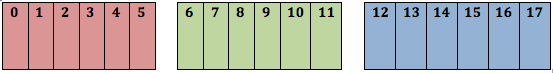
\includegraphics[width=\textwidth]{after_balance.png}
\caption{After load balancing.}
\label{prefix}
\end{figure}


\textbf{ Load Balance Algorithm: }
\begin{itemize}
\item Decide which part of your array belongs to which chare looking at the global rank of your local array.
\begin{itemize}
\item E.g: For Chare 3, local integers have global rank of [5-17]
\item $[5]$ should be in Chare 0 and [6-11] should be in Chare 1 because of FACT \#2.
\end{itemize}
\item Extract values from local array and sent it to the chare together with the index information. 
\begin{itemize}
\item int[values], int $start\_index$, int $end\_index$
\end{itemize}


\item Receiving side: The final array can be pre-allocated according to the average. Whenever a chare receives data, put into the pre-allocated place looking at the index information

\end{itemize}



\textbf{Note:}
\begin{itemize}
\item Store the average as double, not as integer.
\item Even if the avg is not an integer number, the algorithm will still distribute the values evenly, the extra numbers will not be accumulated at the end.
When calculating the index range $[thisIndex(n)*avg, (thisIndex(n)+1)*avg-1]$, the values needs to be rounded down.\\
\end{itemize}


\textbf{Another example showing global index values:}

\begin{figure}[h]
\centering
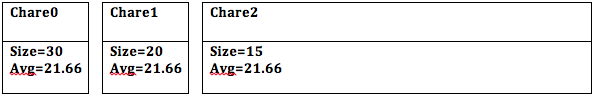
\includegraphics[width=\textwidth]{example.png}
\label{prefix}
\end{figure}
\textbf{Global index values:} $[thisIndex(n)*avg, (thisIndex(n)+1)*avg-1]$\\
Chare 0: [0-20] $->$ 21 values after balance\\
Chare 1: [21-42] $->$ 22 values after balance\\
Chare 2: [43-64] $->$ 22 values after balance\\


\pagebreak


\textbf{Submission:}
Create an mp1 directory in your SVN repository folder and add your code into
that folder and check in the your code.
\begin{itemize}
\item  For each file F you create, that you want to check in, do: \\
        \textit{svn add F}\\
        and frequently (after you have modified F, and have the next better
        version) do:\\ 
        \textit{svn ci F}
\item  There will be a penalty for late submissions.
\end{itemize}

\end{document}
